\documentclass[a4paper,12pt]{report}

% ===================================================
% 1. PAGE SETUP & FONTS
% ===================================================
% Margins: Top=3cm, Bottom=3cm, Left=3.5cm, Right=2cm (Standard TCVN)
\usepackage[a4paper,top=3cm,bottom=3cm,left=3.5cm,right=2cm]{geometry}

% Spacing and Indentation
\usepackage{setspace}
\setstretch{1.5} % 1.5 Line spacing
\usepackage{indentfirst} % Indent the first paragraph of every section
\setlength{\parindent}{0.5cm} % Standard 0.5 inch indent (approx 1.27cm)
\setlength{\parskip}{0pt} % Add a little space between paragraphs for readability

% Fonts: Times New Roman setup
\usepackage{iftex}
\ifPDFTeX
  \usepackage[T5]{fontenc}
  \usepackage[utf8]{inputenc}
  \usepackage{mathptmx} % Times New Roman clone for pdfLaTeX
\else
  \usepackage{fontspec}
  \setmainfont{Times New Roman}
\fi

% Fix font size warnings for non-standard sizes
\usepackage{fix-cm}

% Force the "Normal" font size to 13pt (Standard VN requirement)
\makeatletter
\renewcommand\normalsize{%
   \@setfontsize\normalsize{13pt}{16pt}%
   \abovedisplayskip 12\p@ \@plus3\p@ \@minus7\p@
   \abovedisplayshortskip \z@ \@plus3\p@
   \belowdisplayshortskip 6.5\p@ \@plus3.5\p@ \@minus3\p@
   \belowdisplayskip \abovedisplayskip
   \let\@listi\@listI}
\makeatother
\AtBeginDocument{\normalsize}

% ===================================================
% 2. HEADINGS FORMATTING (The Critical Part)
% ===================================================
\usepackage{titlesec}

% --- CHAPTER (Heading 1) ---
% Format: "CHAPTER X: TITLE" - Centered, Bold, Uppercase, 16pt
\titleformat{\chapter}[block]
  {\centering\normalfont\bfseries\fontsize{16}{19}\selectfont\MakeUppercase} % Format
  {\chaptertitlename\ \thechapter:} % Label (e.g., "CHAPTER 1:")
  {0.5em} % Space between label and title
  {} % Before code

% Adjust spacing around Chapter titles
\titlespacing*{\chapter}{0pt}{-10pt}{20pt} 
% {Left}{Before (negative pulls it up)}{After}

% --- SECTION (Heading 2) ---
% Format: "1.1 Title" - Left, Bold, 13pt
\titleformat{\section}
  {\normalfont\bfseries\fontsize{13}{16}\selectfont}
  {\thesection}{1em}{}
\titlespacing*{\section}{0pt}{12pt}{6pt}

% --- SUBSECTION (Heading 3) ---
% Format: "1.1.1 Title" - Left, Bold, 13pt
\titleformat{\subsection}
  {\normalfont\bfseries\fontsize{13}{16}\selectfont}
  {\thesubsection}{1em}{}
\titlespacing*{\subsection}{0pt}{12pt}{6pt}

% --- SUBSUBSECTION (Heading 4) ---
% Format: "1.1.1.1 Title" - Left, Italic, 13pt
\titleformat{\subsubsection}
  {\normalfont\itshape\fontsize{13}{16}\selectfont}
  {\thesubsubsection}{1em}{}
\titlespacing*{\subsubsection}{0pt}{12pt}{6pt}

% Numbering depth
\setcounter{secnumdepth}{4}
\setcounter{tocdepth}{3}

% ===================================================
% 3. CAPTIONS & REFERENCES
% ===================================================
\usepackage{graphicx}
\usepackage{tikz}
\usetikzlibrary{calc}
\usepackage{caption}
\usepackage{float} % provides the [H] placement option
\usepackage{xurl} % allow URL line breaks to fix overfull \hbox
\usepackage[hidelinks]{hyperref}
\usepackage{listings}
\usepackage{listingsutf8}
\usepackage{xcolor}
\usepackage{enumitem}

% Define colors for code listings
\definecolor{codegray}{rgb}{0.9,0.9,0.9}
\lstset{
    backgroundcolor=\color{codegray},
    basicstyle=\ttfamily\small,
    breaklines=true,
    frame=single,
    rulecolor=\color{lightgray},
    showstringspaces=false,
    inputencoding=utf8,
    extendedchars=true
}

% Caption styling: Label Bold, Text Italic
\captionsetup{labelfont=bf,textfont=it,labelsep=colon}

% --- LANGUAGE SETTINGS ---
% UNCOMMENT the pair you need:

% OPTION A: ENGLISH (Standard)
% \renewcommand{\chaptername}{CHAPTER}
% \renewcommand{\figurename}{Figure}
% \renewcommand{\tablename}{Table}
% \renewcommand{\contentsname}{TABLE OF CONTENTS}

% OPTION B: VIETNAMESE (Standard)
\renewcommand{\chaptername}{CHƯƠNG}
\renewcommand{\figurename}{Hình}
\renewcommand{\tablename}{Bảng}
\renewcommand{\contentsname}{MỤC LỤC}
\renewcommand{\listfigurename}{DANH MỤC HÌNH ẢNH}

% ===================================================
% 4. HEADER & FOOTER
% ===================================================
\usepackage{fancyhdr}
\pagestyle{fancy}
\fancyhf{}
\fancyfoot[C]{\thepage} % Page number bottom center
\renewcommand{\headrulewidth}{0pt} % No line at top
\renewcommand{\footrulewidth}{0pt}

% ===================================================
% DOCUMENT BEGINS
% ===================================================
\begin{document}

% --- TITLE PAGE ---
\begin{titlepage}
\begin{tikzpicture}[remember picture, overlay]
    \draw[line width = 4.5pt] ($(current page.north west) + (3.0cm,-2.0cm)$) rectangle ($(current page.south east) + (-2.0cm,2.0cm)$);
\end{tikzpicture}

\centering
\vspace*{0.5cm}
{\fontsize{13}{15}\selectfont \textbf{ĐẠI HỌC CẦN THƠ}\par}
{\fontsize{13}{15}\selectfont \textbf{TRƯỜNG CÔNG NGHỆ THÔNG TIN \& TRUYỀN THÔNG}\par}

\vspace{0.5cm}
\begin{figure}[h]
    \centering
    
\includegraphics[width=3cm]{./assets/logo-ctu.png}
\end{figure}
\vspace{0.5cm}

{\fontsize{18}{22}\selectfont \textbf{BÁO CÁO}\par}
{\fontsize{18}{22}\selectfont \textbf{PHÁT TRIỂN ỨNG DỤNG WEB}\par}
{\fontsize{18}{22}\selectfont \textbf{CT449}\par}

\vspace{1cm}

{\fontsize{13}{15}\selectfont \textbf{Bài Tập}\par}
{\fontsize{20}{24}\selectfont \textbf{FRONTEND}\par}

\vspace{2cm}

\begin{flushleft}
\hspace{2cm}
\begin{tabular}{ll}
\textbf{Giảng viên hướng dẫn:} & Ths. Nguyễn Minh Trung \\
\textbf{Sinh viên thực hiện:} & Trần Thanh Duy \\
\textbf{MSSV:} & DC24V7X604 \\
\end{tabular}
\end{flushleft}

\vfill
{\fontsize{13}{15}\selectfont \textbf{Cần Thơ, năm 2026}\par}
\end{titlepage}

% --- FRONT MATTER ---
\pagenumbering{roman} % i, ii, iii...

\phantomsection
\addcontentsline{toc}{chapter}{\contentsname}
\tableofcontents
\clearpage

\phantomsection
\addcontentsline{toc}{chapter}{\listfigurename}
\listoffigures
\clearpage

% --- MAIN CONTENT ---
\pagenumbering{arabic} % 1, 2, 3...
\setcounter{page}{1}

% CHAPTER 1
\chapter{ỨNG DỤNG CONTACTBOOK - FRONTEND} % Will automatically print "CHAPTER 1: INTRODUCTION"
\section{Tạo dự án và cấu hình môi trường}

Tạo dự án contactbook-frontend bằng lệnh \texttt{npm create vue@latest}.

Vào thư mục dự án, XÓA bỏ nội dung thư mục src/components và hiệu chỉnh tập tin App.vue như sau:

\begin{figure}[H]
    \centering
    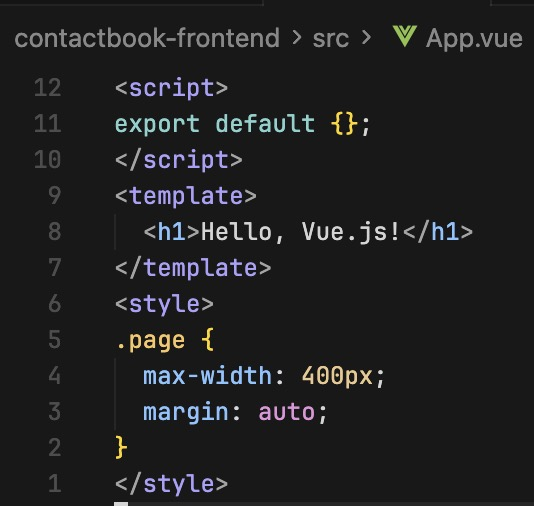
\includegraphics[width=0.6\textwidth]{./assets/appvue.jpg}
    \caption{Hiệu chỉnh App.vue}
    \label{fig:appvue}
\end{figure}

Hiệu chỉnh tập tin vite.config.js để cấu hình port cho ứng dụng:

\begin{figure}[H]
    \centering
    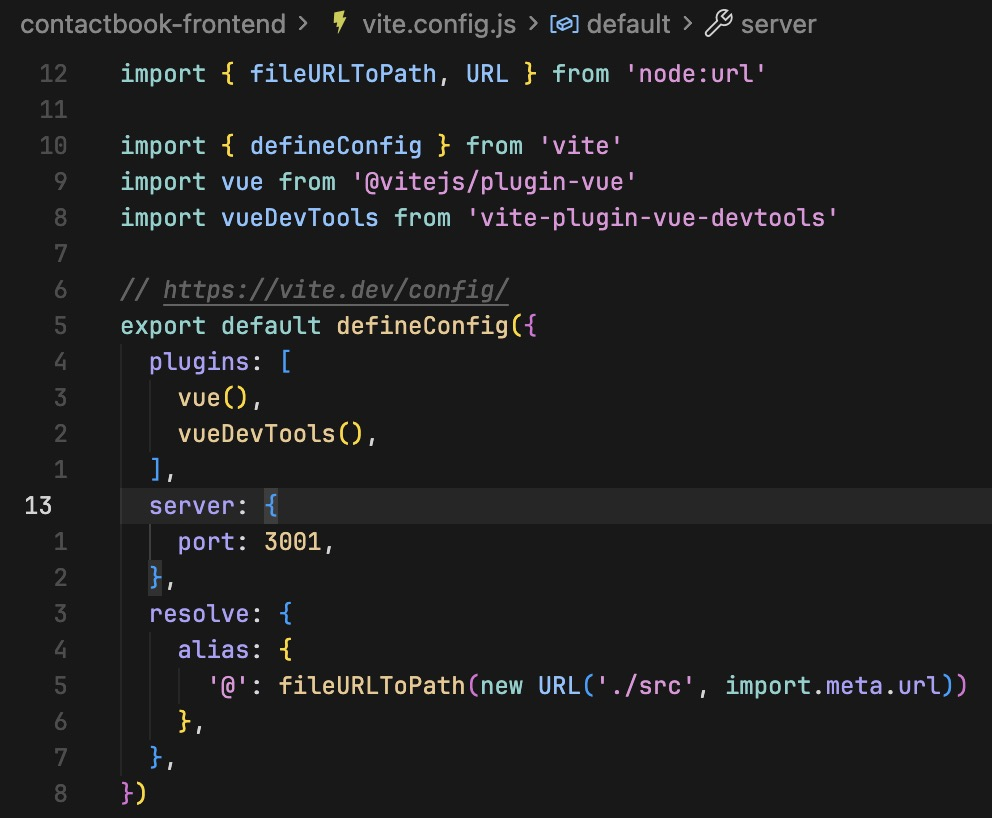
\includegraphics[width=0.8\textwidth]{./assets/viteconfig.jpg}
    \caption{Cấu hình vite.config.js}
    \label{fig:viteconfig}
\end{figure}

Thực hiện cài đặt các package cần thiết bằng lệnh \texttt{npm install}.

Khởi động server bằng lệnh \texttt{npm run dev}.

\begin{figure}[H]
    \centering
    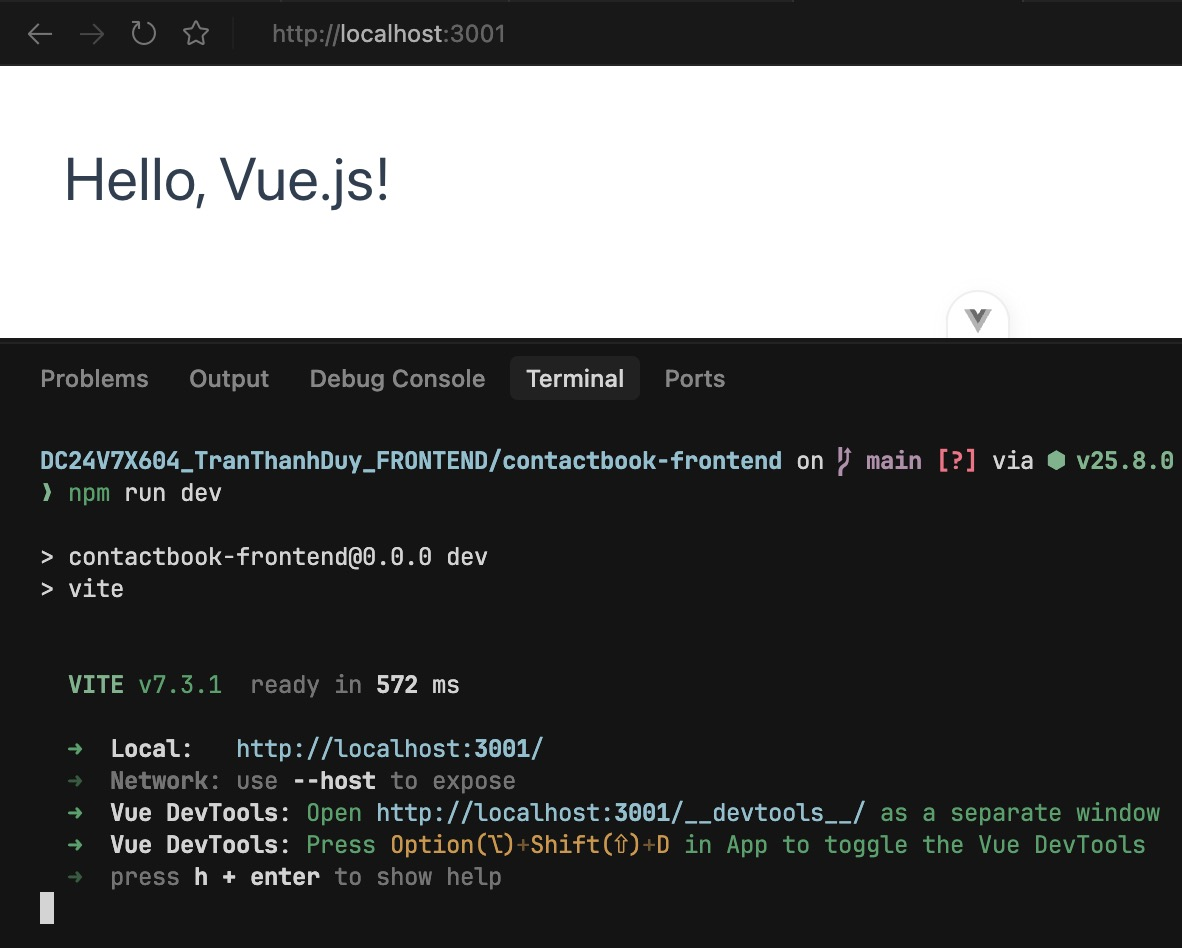
\includegraphics[width=0.7\textwidth]{./assets/hellovue.jpg}
    \caption{Khởi động server}
    \label{fig:server}
\end{figure}


% Chỉnh sửa app.js
% \begin{lstlisting}
% ...
% import ApiError from "./app/api-error.js";  
% ...
% // handle 404 error
% app.use((req, res, next) => {
%   return next(new ApiError(404, "Resource not found"));
% });

% // define error-handling middleware last, after other app.use() and routes calls
% app.use((err, req, res, next) => {
%   return res.status(err.statusCode || 500).json({
%     message: err.message || "Internal Server Error",
%   });
% }); 
% \end{lstlisting}

% \section{Cấu trúc thư mục dự án đến thời điểm này}

% \begin{figure}[H]
%   \centering
%   
\includegraphics[width=0.4\textwidth]{./assets/img18.jpg}
%   \caption{Cấu trúc thư mục dự án}
%   \label{fig:project_structure}
% \end{figure}

% \section{Link Github}

% \url{https://github.com/duytechie/DC24V7X604_TranThanhDuy_BACKEND_1}

\section{Tạo lớp dịch vụ lấy dữ liệu từ server}

Tạo tập tin src/services/api.service.js với nội dung sau:

\begin{figure}[H]
    \centering
    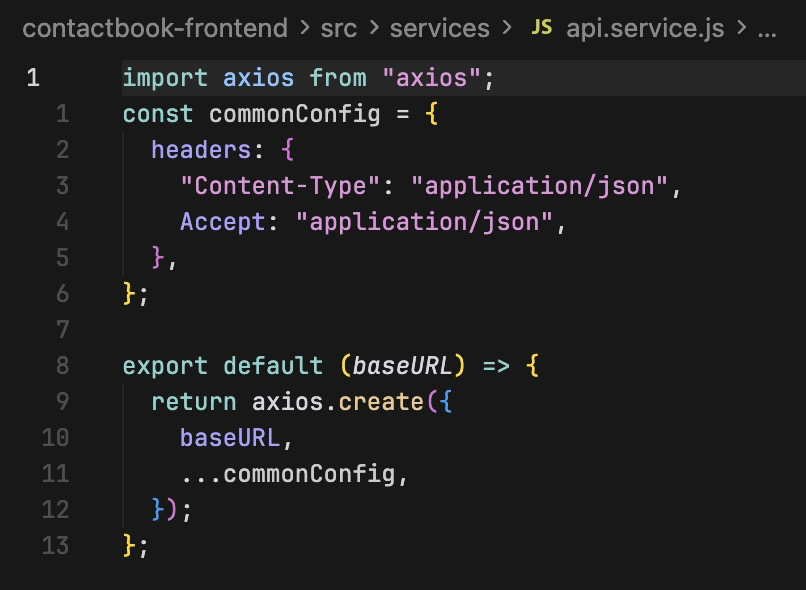
\includegraphics[width=0.6\textwidth]{./assets/api_service.png}
    \caption{Lớp dịch vụ api.service.js}
    \label{fig:apiservice}
\end{figure}

Tạo tập tin src/services/contact.service.js với nội dung sau:

\begin{figure}[H]
    \centering
    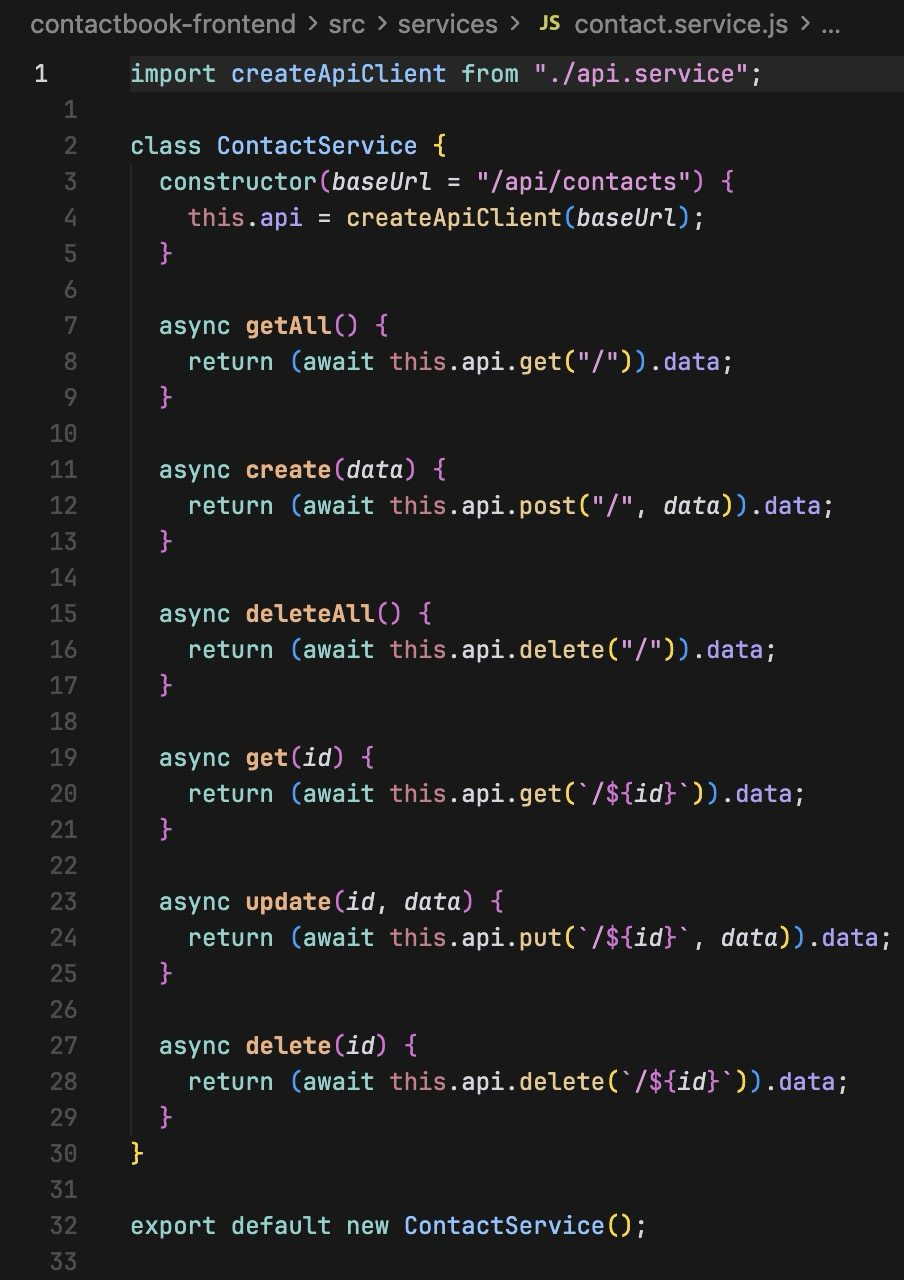
\includegraphics[width=0.5\textwidth]{./assets/contact_service.png}
    \caption{Lớp dịch vụ contact.service.js}
    \label{fig:contactservice}
\end{figure}

Cấu hình vite.config.js để proxy đến server:
\begin{figure}[H]
    \centering
    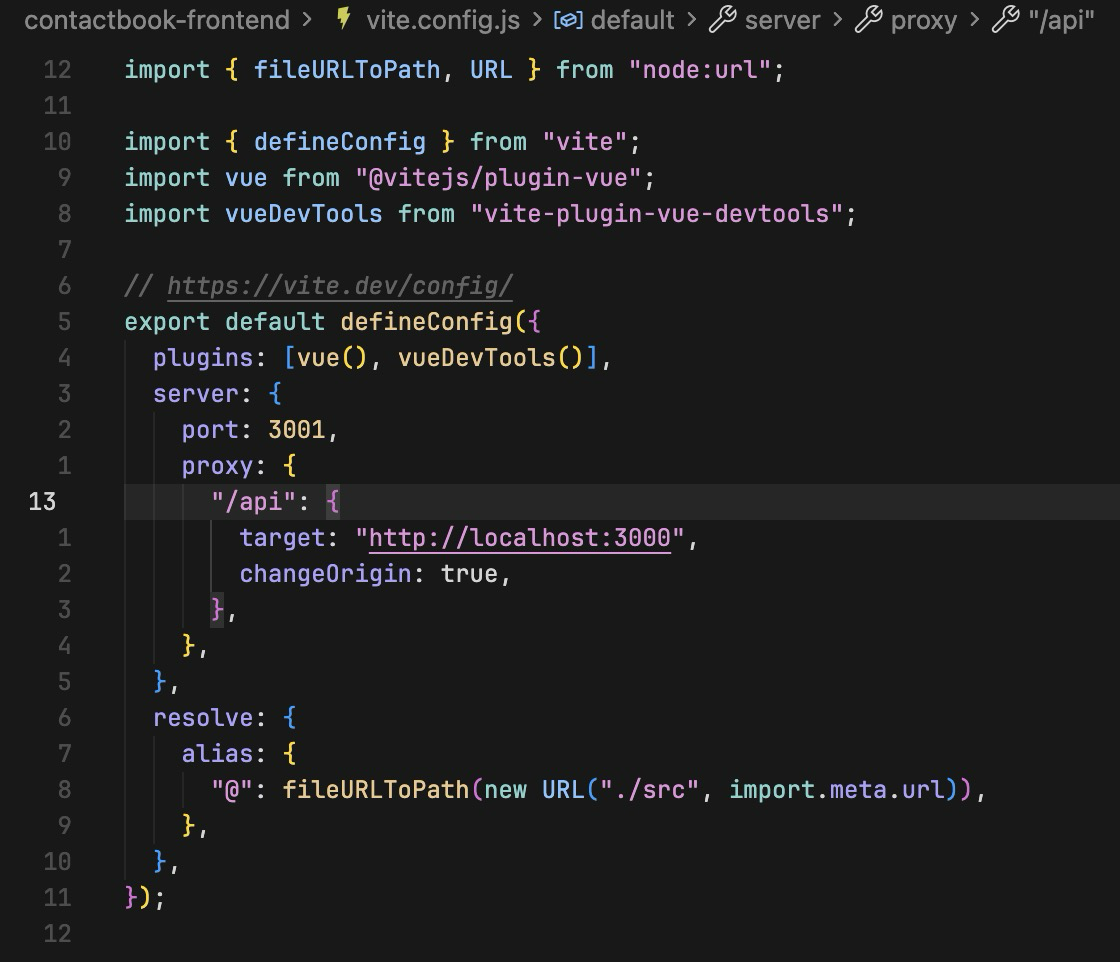
\includegraphics[width=0.8\textwidth]{./assets/vite_proxy.png}
    \caption{Cấu hình proxy đến server}
    \label{fig:viteproxy}
\end{figure}

\section{Cài đặt trang hiển thị danh sách các liên hệ}
  
Xem url git commit để biết thêm chi tiết:
\begin{itemize}[noitemsep, topsep=0pt, partopsep=0pt, parsep=0pt]
    \item \href{https://github.com/duytechie/DC24V7X604_TranThanhDuy_FRONTEND/commit/f6aac04c2b83faca36045dce3bccbf813727b85c}{f6aac04}
    \item \href{https://github.com/duytechie/DC24V7X604_TranThanhDuy_FRONTEND/commit/45821250458e71a310632174f512c3d26cf11376}{4582125}
    \item \href{https://github.com/duytechie/DC24V7X604_TranThanhDuy_FRONTEND/commit/4da046437886b5ee7091eba57ed3ba5fa4f7b89e}{4da0464}
\end{itemize}

\begin{figure}[H]
    \centering
    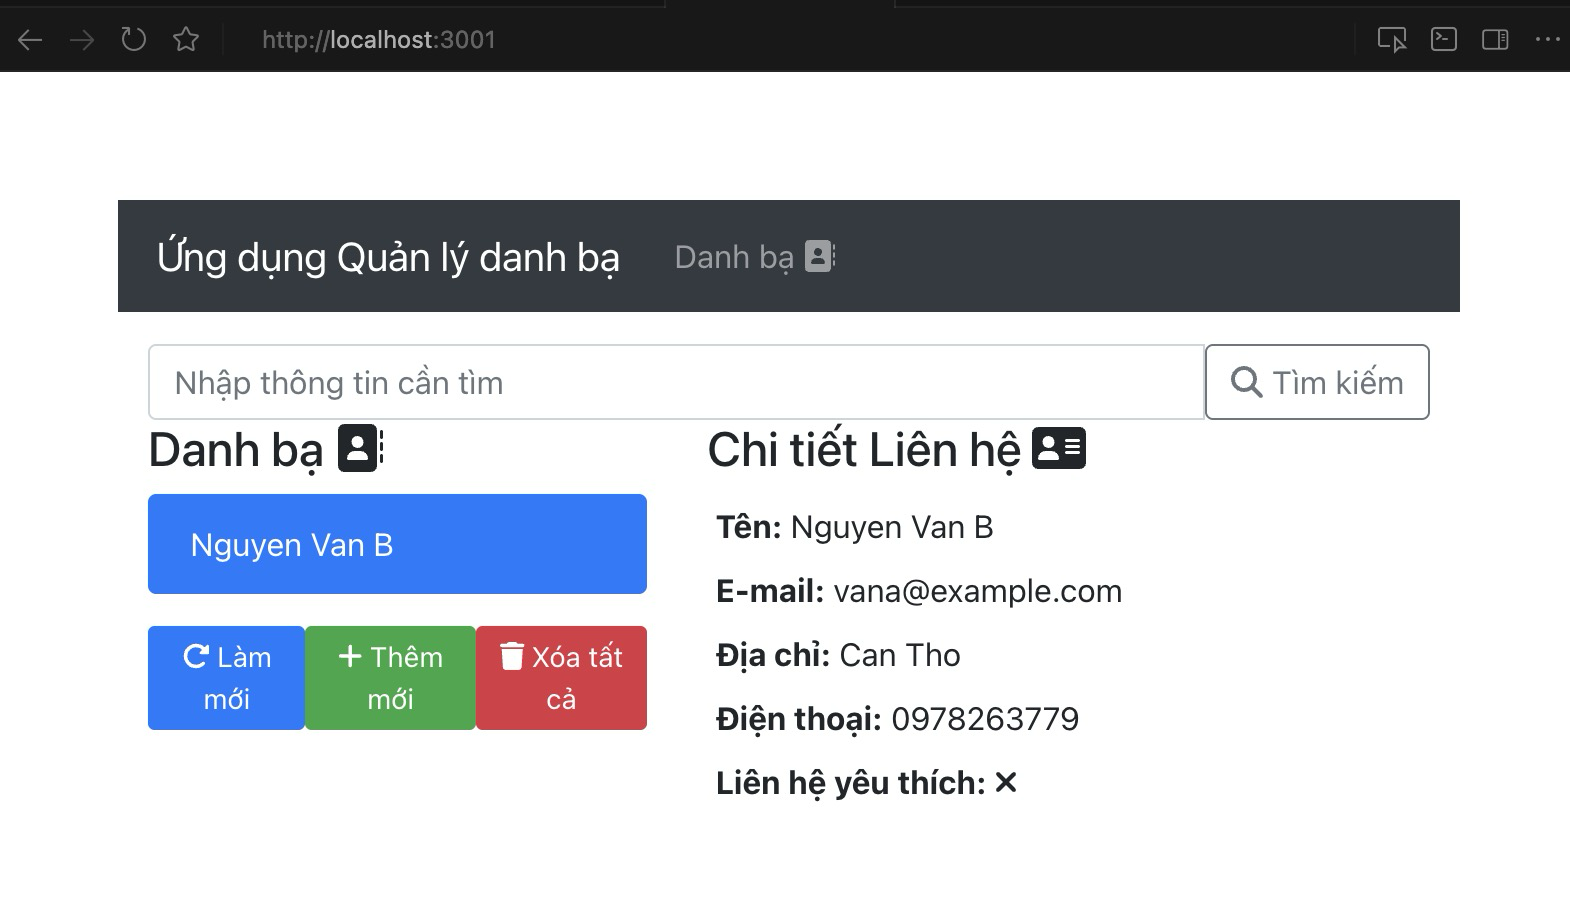
\includegraphics[width=0.8\textwidth]{./assets/step4_result.png}
    \caption{Kết quả trang hiển thị danh sách các liên hệ}
    \label{fig:step4_result}
\end{figure}

\section{Tạo trang lỗi 404 không tìm thấy trang}

Chỉnh sửa index.js và NotFound.vue như sau:

\begin{figure}[H]
    \centering
    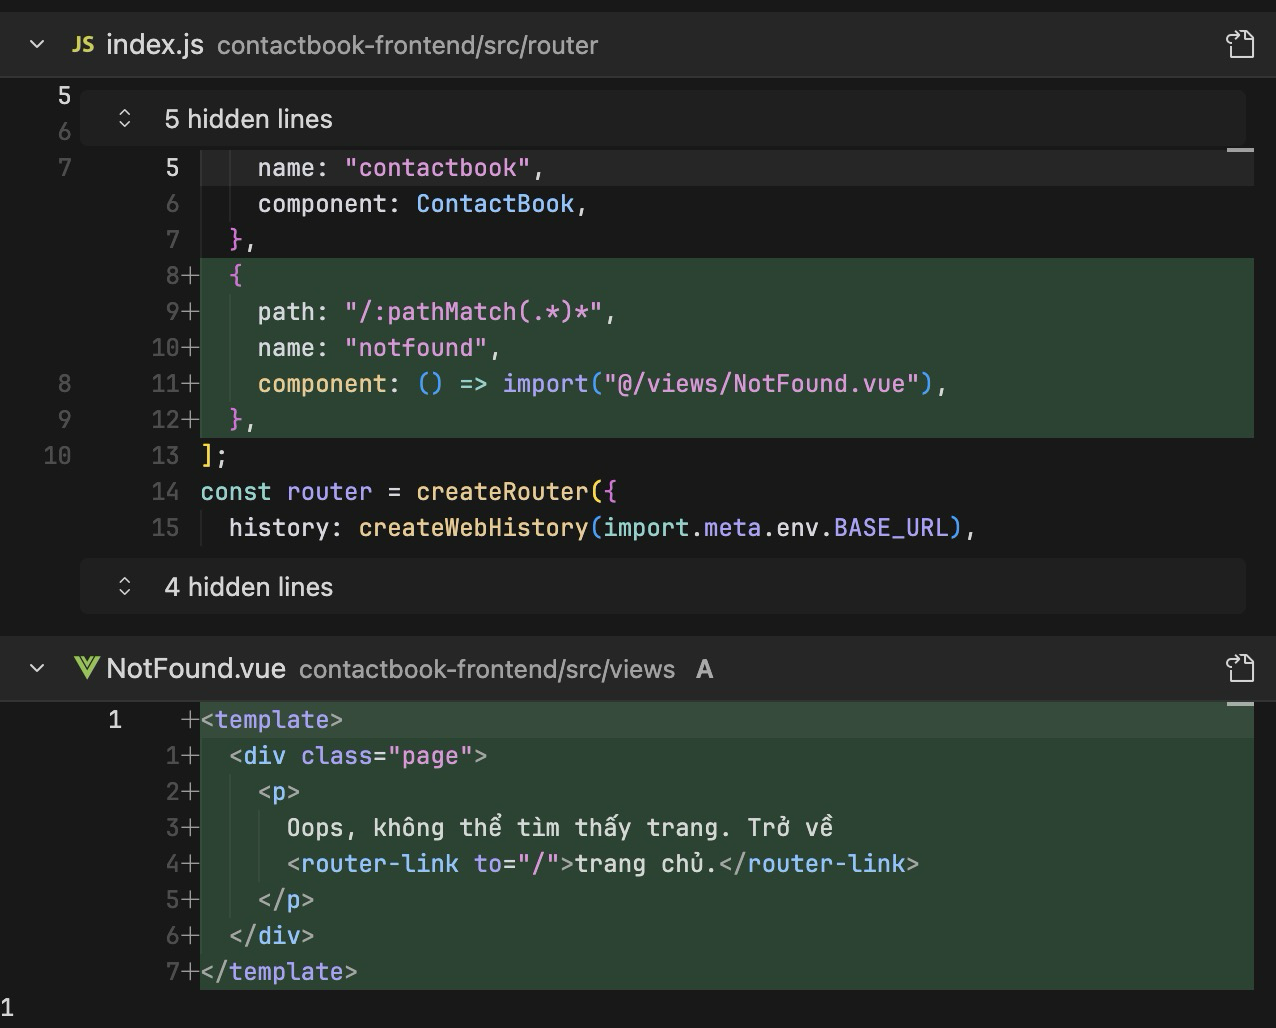
\includegraphics[width=0.8\textwidth]{./assets/code_404.png}
    \caption{Chỉnh sửa index.js và NotFound.vue}
    \label{fig:code_404}
\end{figure}

Kết quả:
\begin{figure}[H]
    \centering
    
\includegraphics[width=0.8\textwidth]{./assets/step5_result.png}
    \caption{Kết quả trang lỗi 404 không tìm thấy trang}
    \label{fig:step5_result}
\end{figure}

\section{Tạo form để thêm hoặc cập nhật liên hệ}

Sao chép tập tin form.css đã cho vào thư mục src/assets/ sau đó tạo tập tin ContactForm.vue trong thư mục
src/components/ với nội dung sau:

\lstinputlisting[inputencoding=utf8/latin1]{./assets/ContactForm.vue}

\section{Tạo trang cập nhật liên hệ}

Tạo tập tin src/views/ContactEdit.vue sau đó chỉnh sửa tập tin ContactBook.vue và index.js như sau:

\begin{figure}[H]
    \centering
    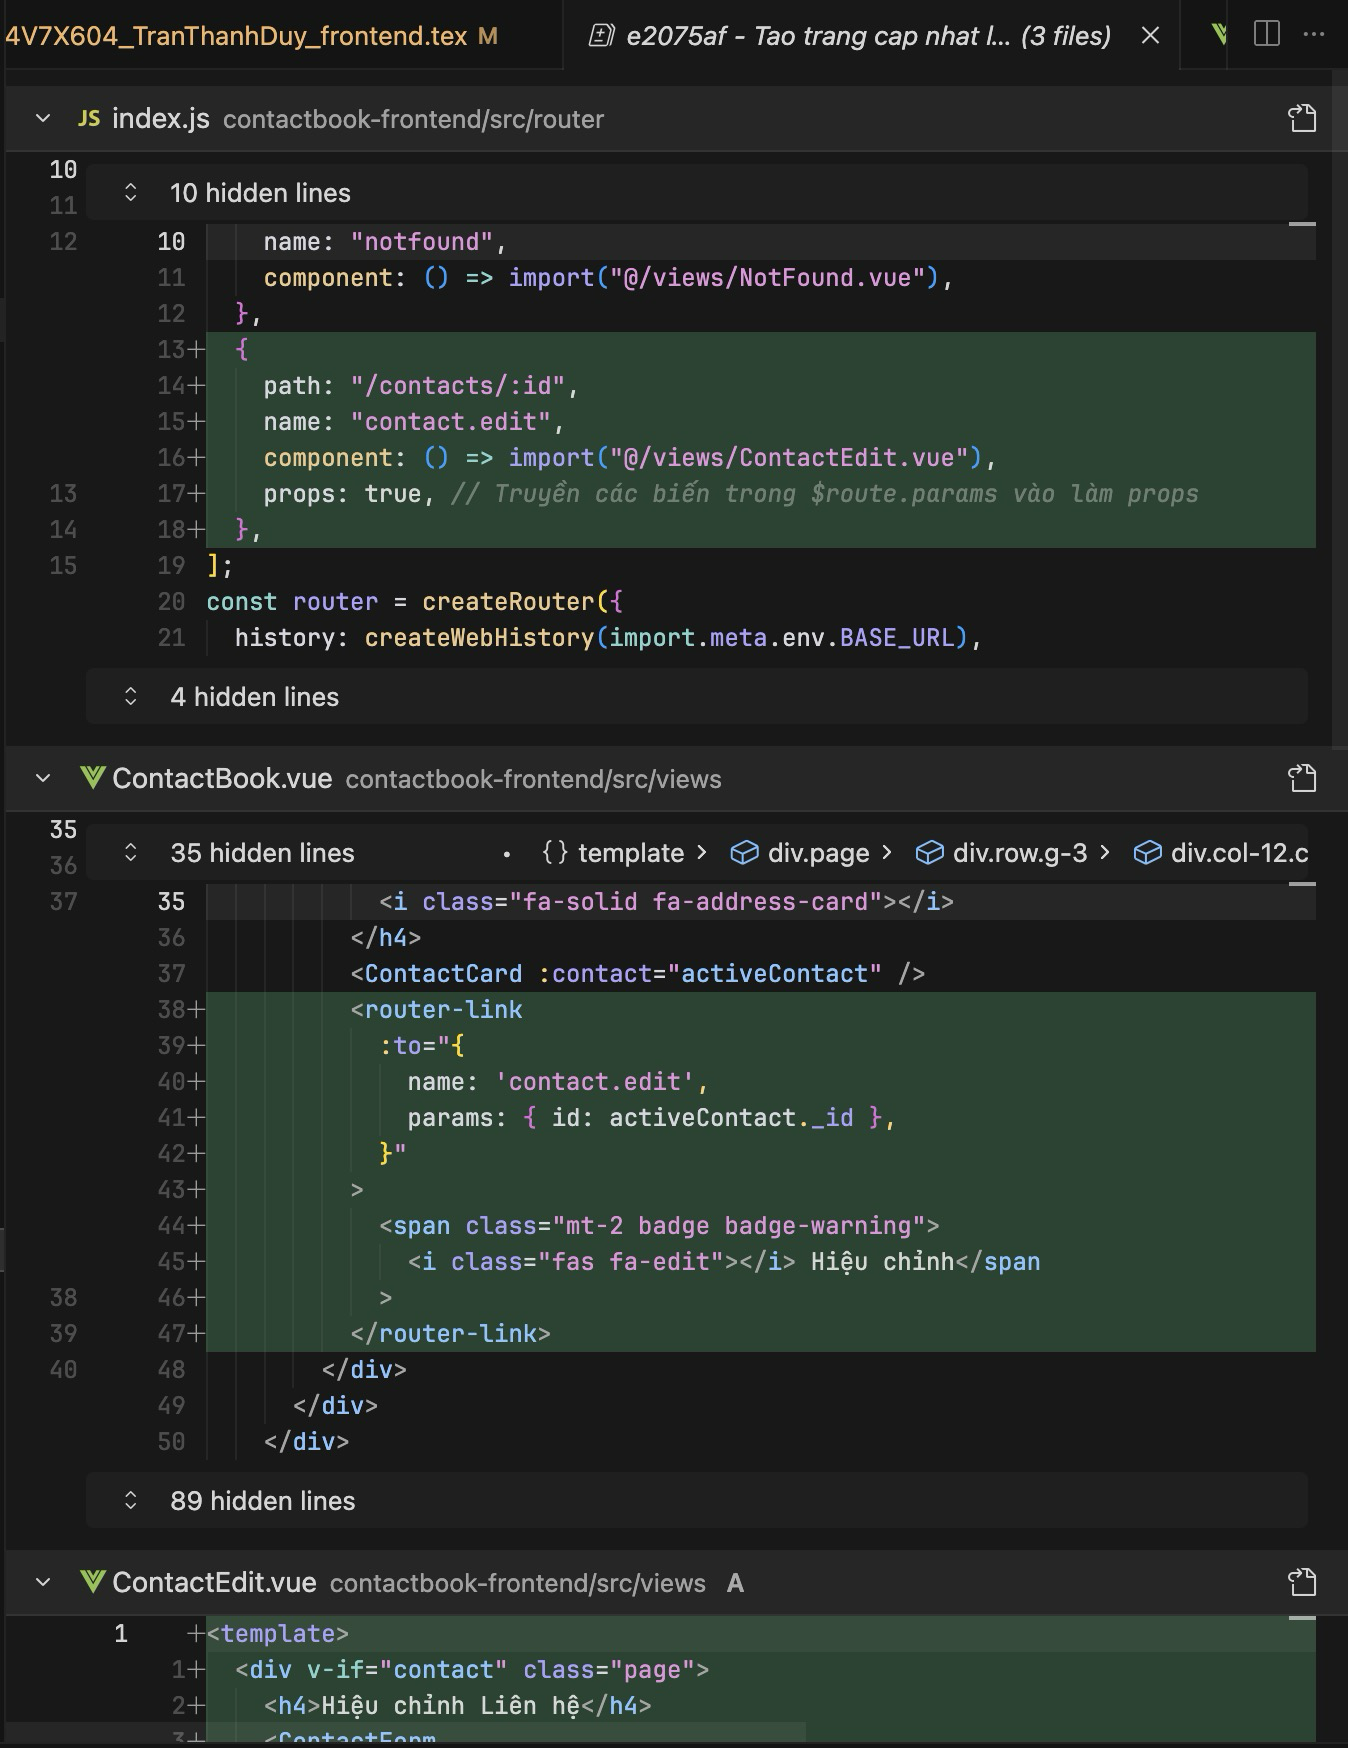
\includegraphics[width=0.8\textwidth]{./assets/contact_update_code.png}
    \caption{Code tạo trang cập nhật liên hệ}
    \label{fig:contact_update_code}
\end{figure}

Xem url git commit để biết thêm chi tiết:
\begin{itemize}[noitemsep, topsep=0pt, partopsep=0pt, parsep=0pt]
    \item \href{https://github.com/duytechie/DC24V7X604_TranThanhDuy_FRONTEND/commit/e2075afb9e59b3b083bf7d137d2d054d137f5c03}{e2075af}
\end{itemize}

Kết quả:
Trang cập nhật liên hệ:
\begin{figure}[H]
    \centering
    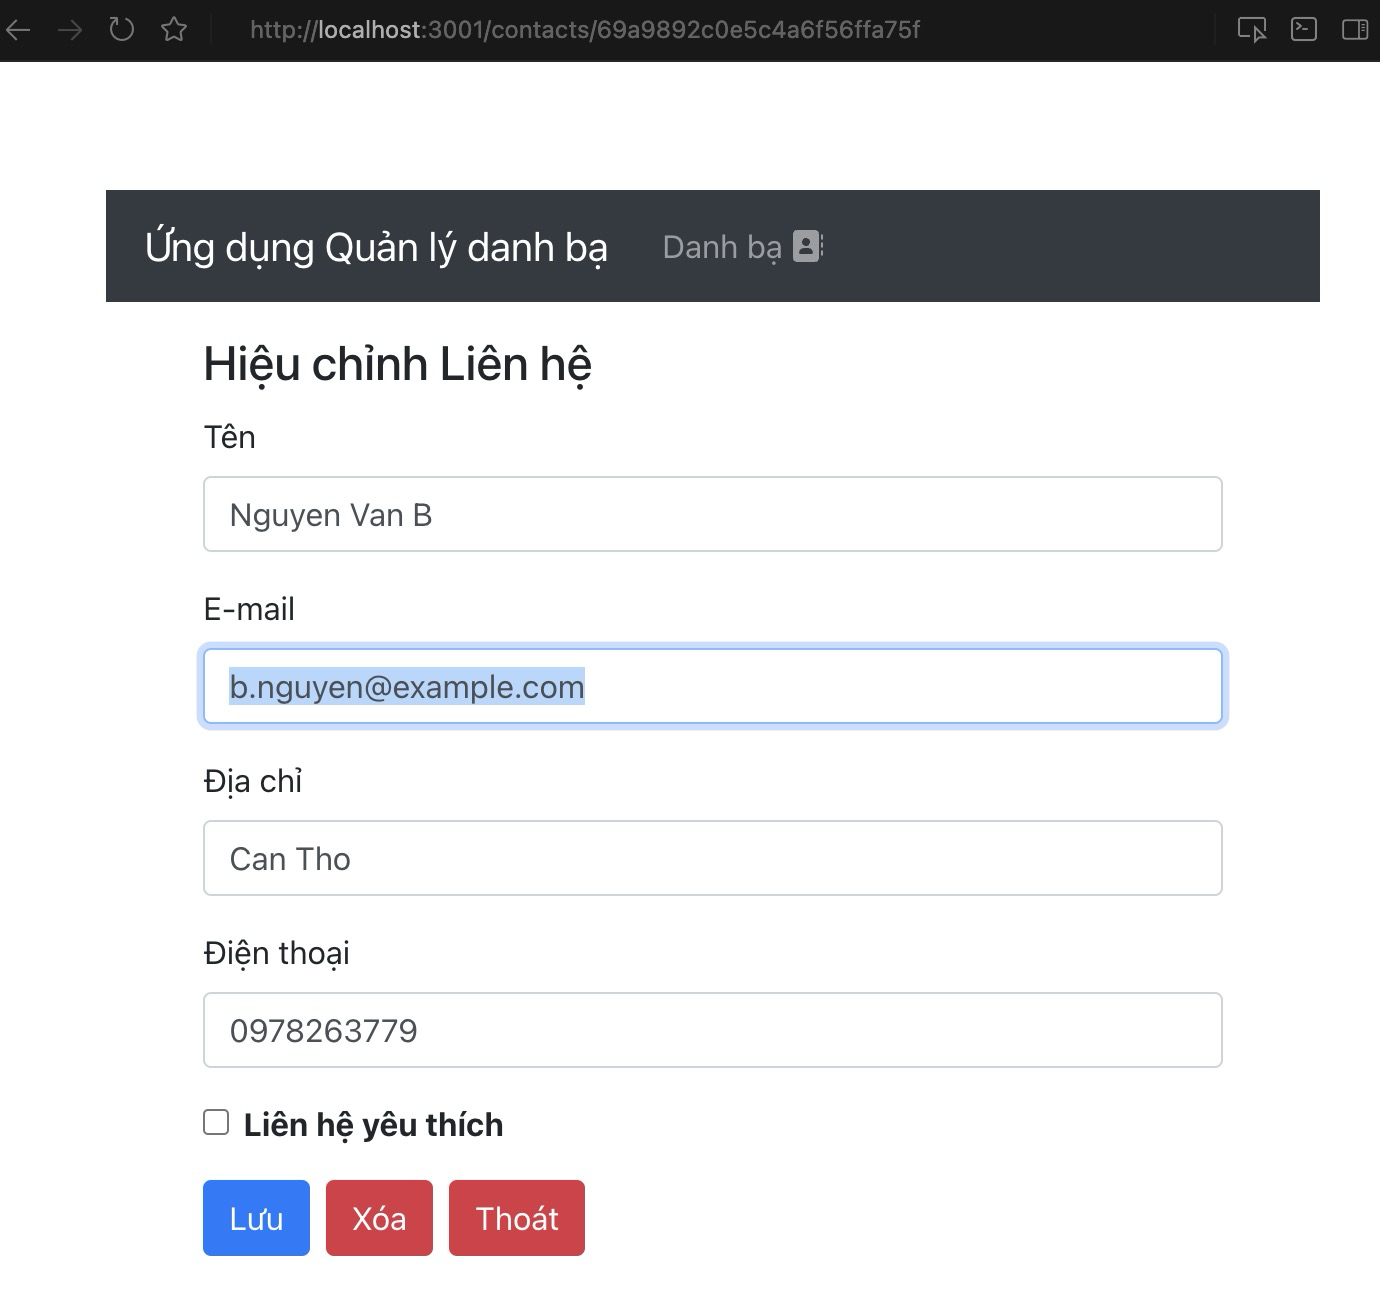
\includegraphics[width=0.6\textwidth]{./assets/contact_update.png}
    \caption{Trang cập nhật liên hệ}
    \label{fig:contact_update_page}
\end{figure}

Sau khi cập nhật liên hệ, trang sẽ được cập nhật lại và hiển thị thông tin liên hệ mới nhất
\begin{figure}[H]
    \centering
    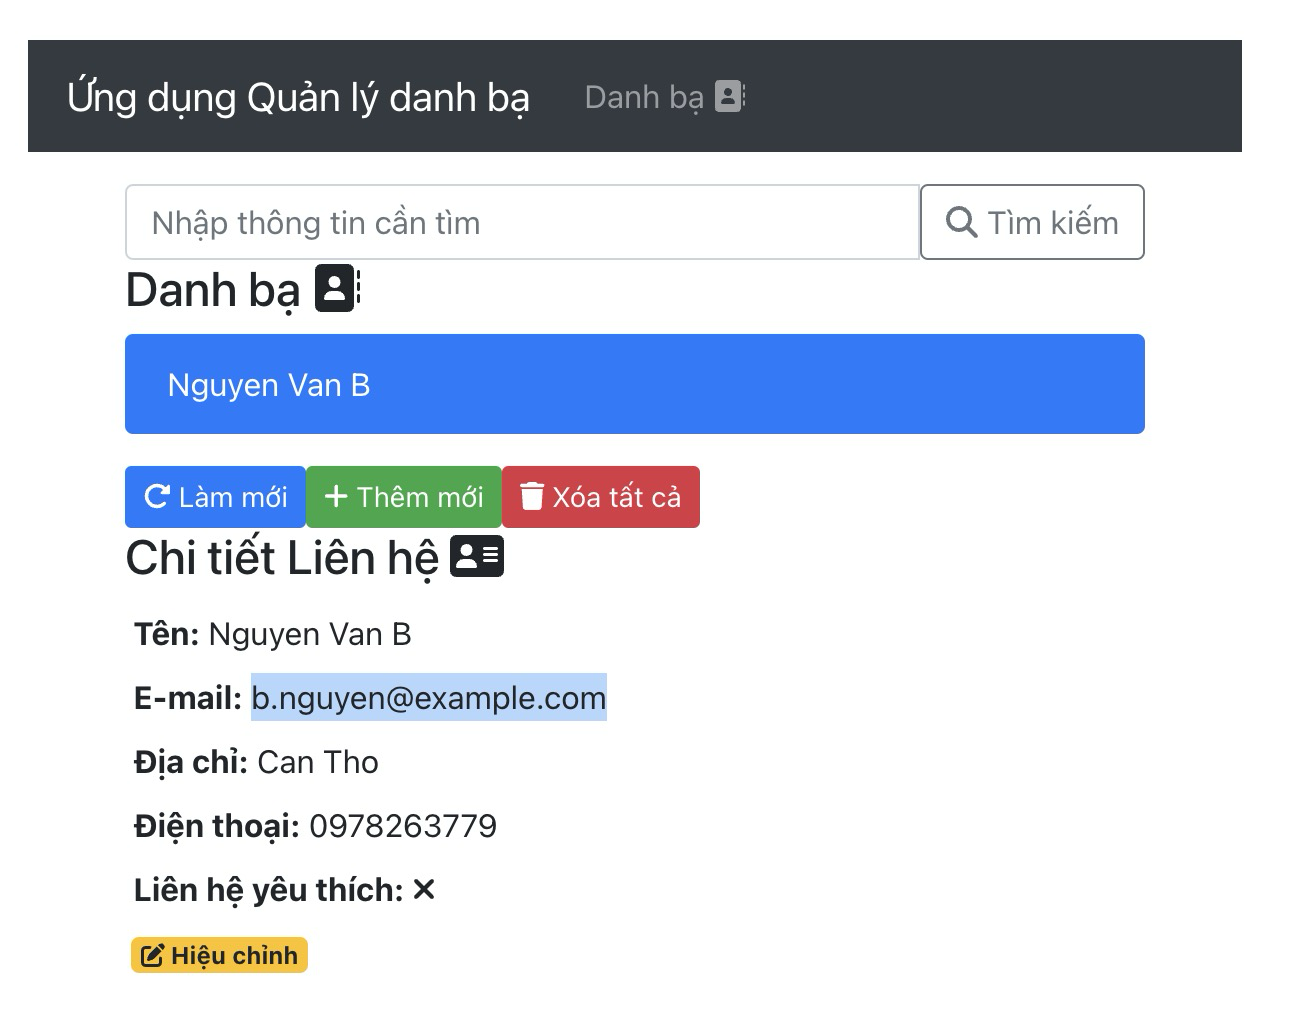
\includegraphics[width=0.6\textwidth]{./assets/contact_update_result.png}
    \caption{Kết quả trang cập nhật liên hệ}
    \label{fig:contact_update_result}
\end{figure}

\section{Tạo trang thêm mới một liên hệ}

Tạo tập tin src/views/ContactAdd.vue sau đó chỉnh sửa tập tin index.js như sau:

\begin{figure}[H]
    \centering
    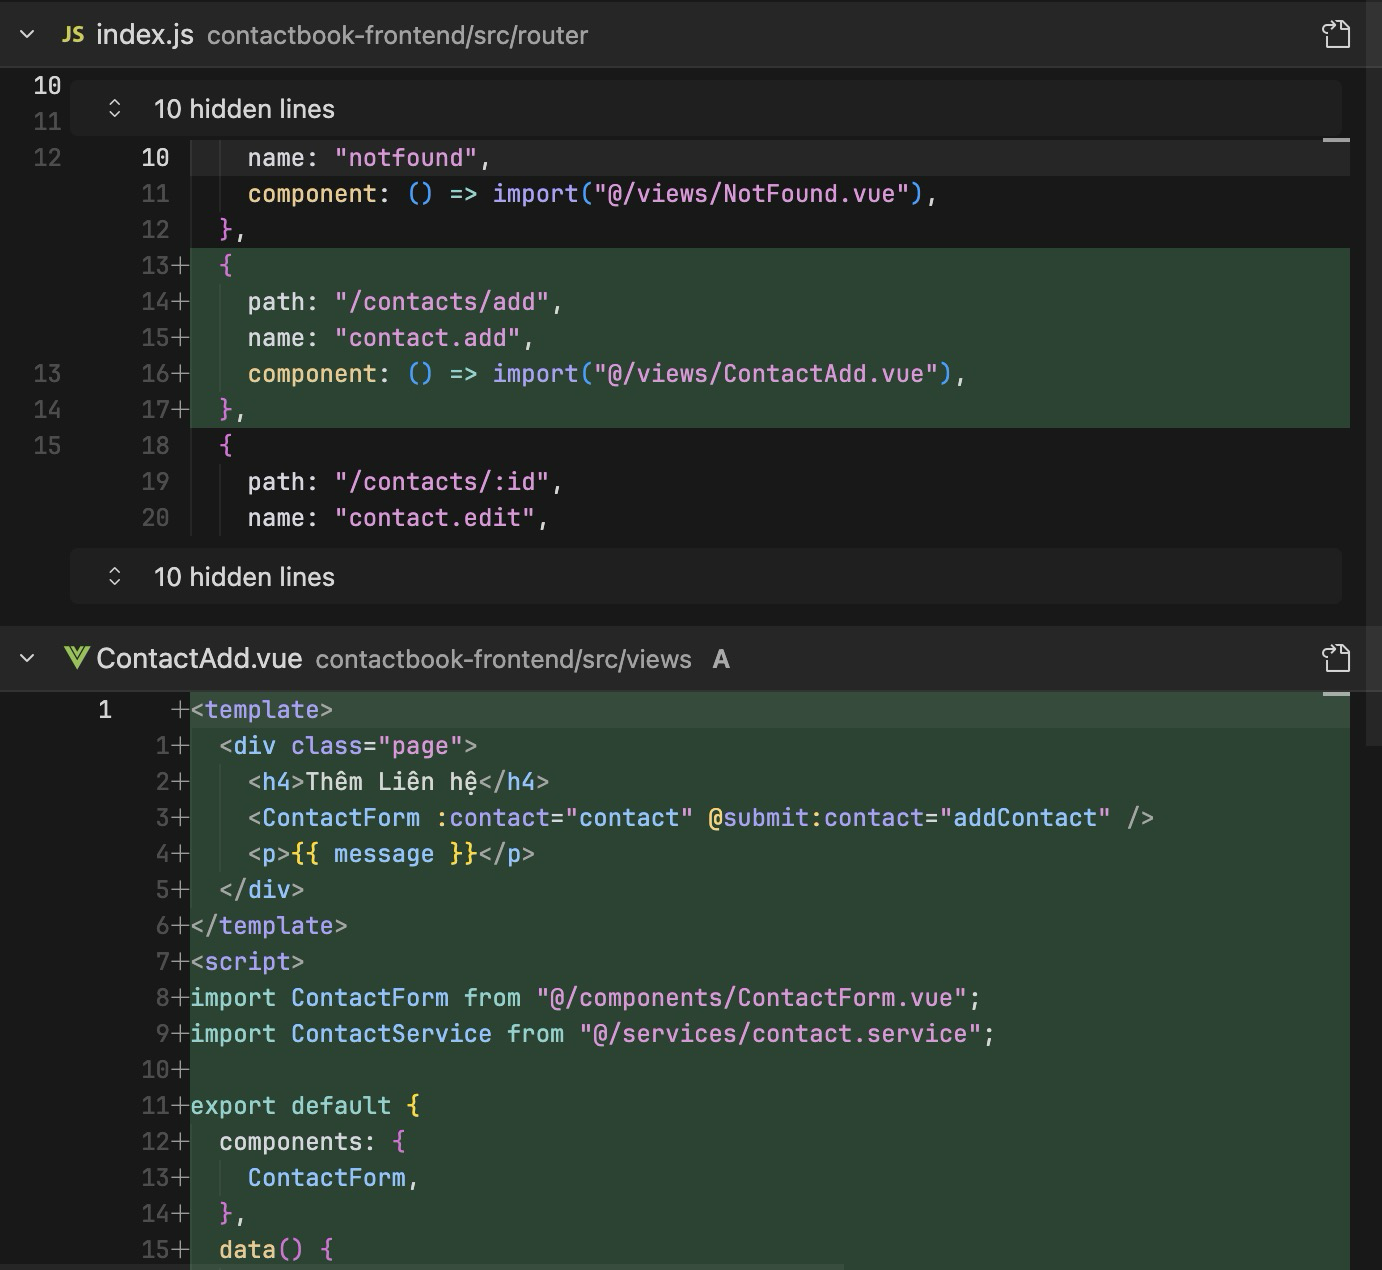
\includegraphics[width=0.8\textwidth]{./assets/contact_add_code.png}
    \caption{Code tạo trang thêm mới một liên hệ}
    \label{fig:contact_add_code}
\end{figure}

Xem url git commit để biết thêm chi tiết:
\begin{itemize}[noitemsep, topsep=0pt, partopsep=0pt, parsep=0pt]
    \item \href{https://github.com/duytechie/DC24V7X604_TranThanhDuy_FRONTEND/commit/f277cb6a0e7d44892125d324efa3d4e1f976bc4a}{f277cb6}
\end{itemize}

Kết quả:
Trang thêm mới một liên hệ:
\begin{figure}[H]
    \centering
    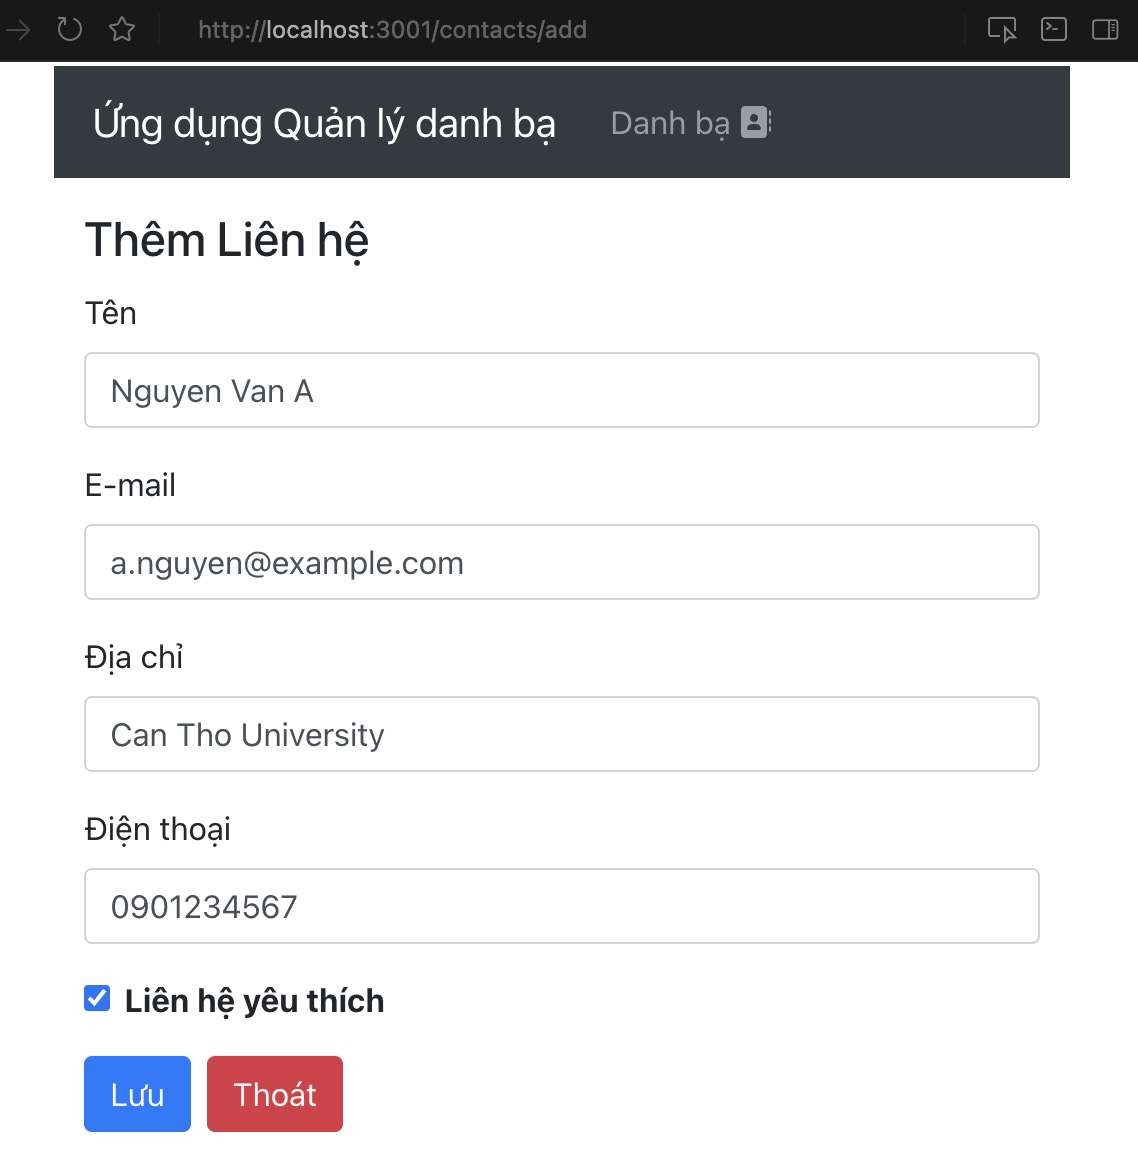
\includegraphics[width=0.4\textwidth]{./assets/contact_add_form.png}
    \caption{Trang thêm mới một liên hệ}
    \label{fig:contact_add_page}
\end{figure}

Sau khi thêm mới liên hệ, trang sẽ được cập nhật lại và hiển thị thông tin liên hệ mới nhất
\begin{figure}[H]
    \centering
    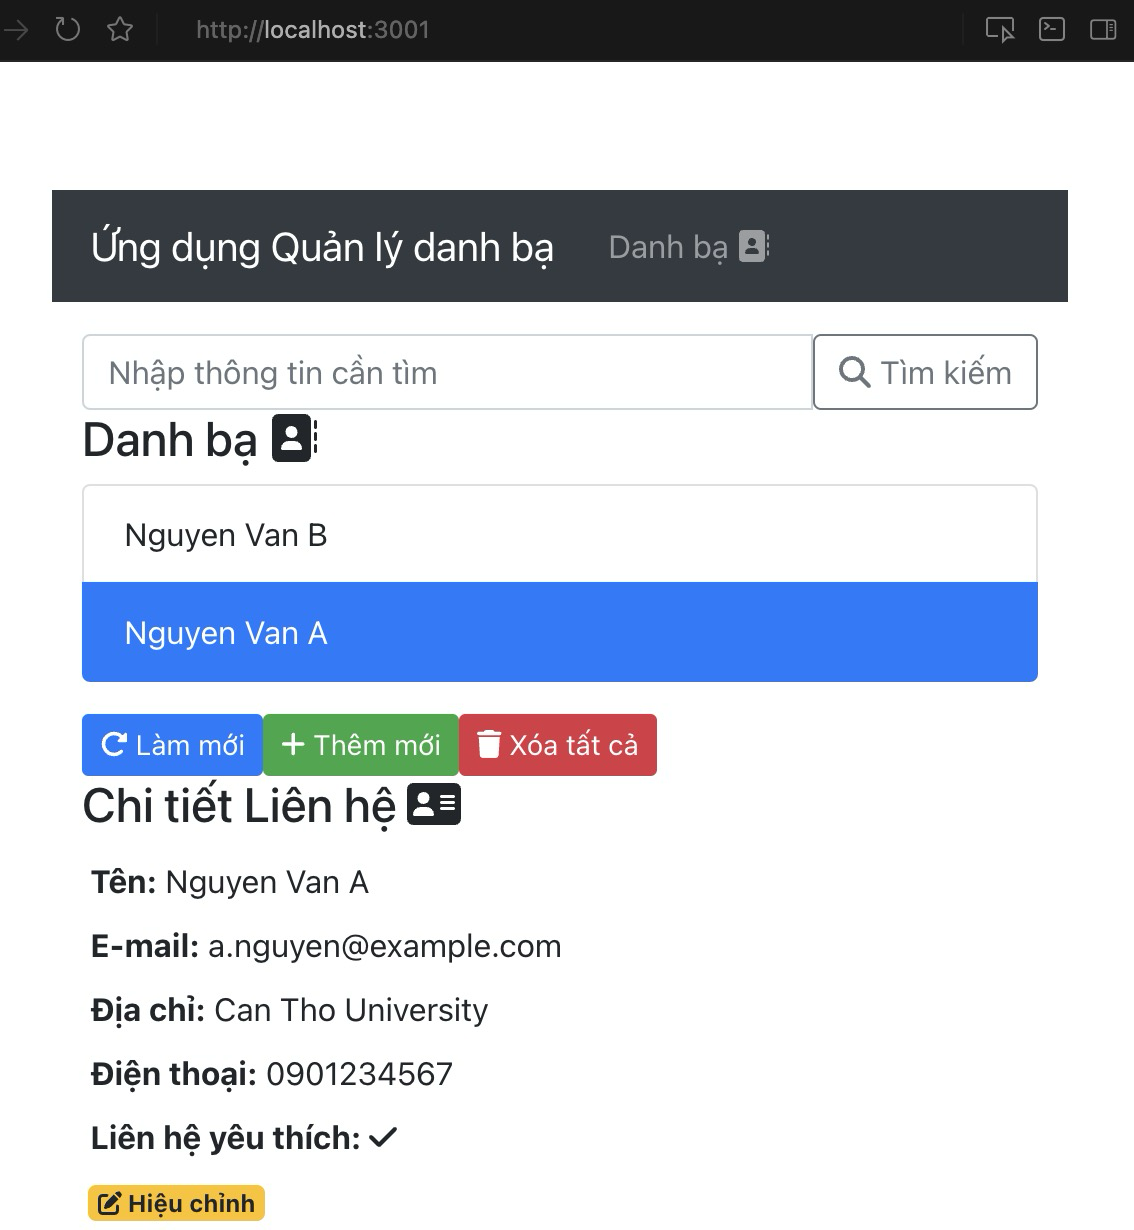
\includegraphics[width=0.6\textwidth]{./assets/contact_add_result.png}
    \caption{Kết quả trang thêm mới một liên hệ}
    \label{fig:contact_add_result}
\end{figure}

\section{Phần mở rộng: Tạo trang đăng nhập}

Tạo tập tin LoginView.vue và auth.service.js, sau đó chỉnh sửa tập tin index.js, AppHeader.vue như sau:

\begin{figure}[H]
    \centering
    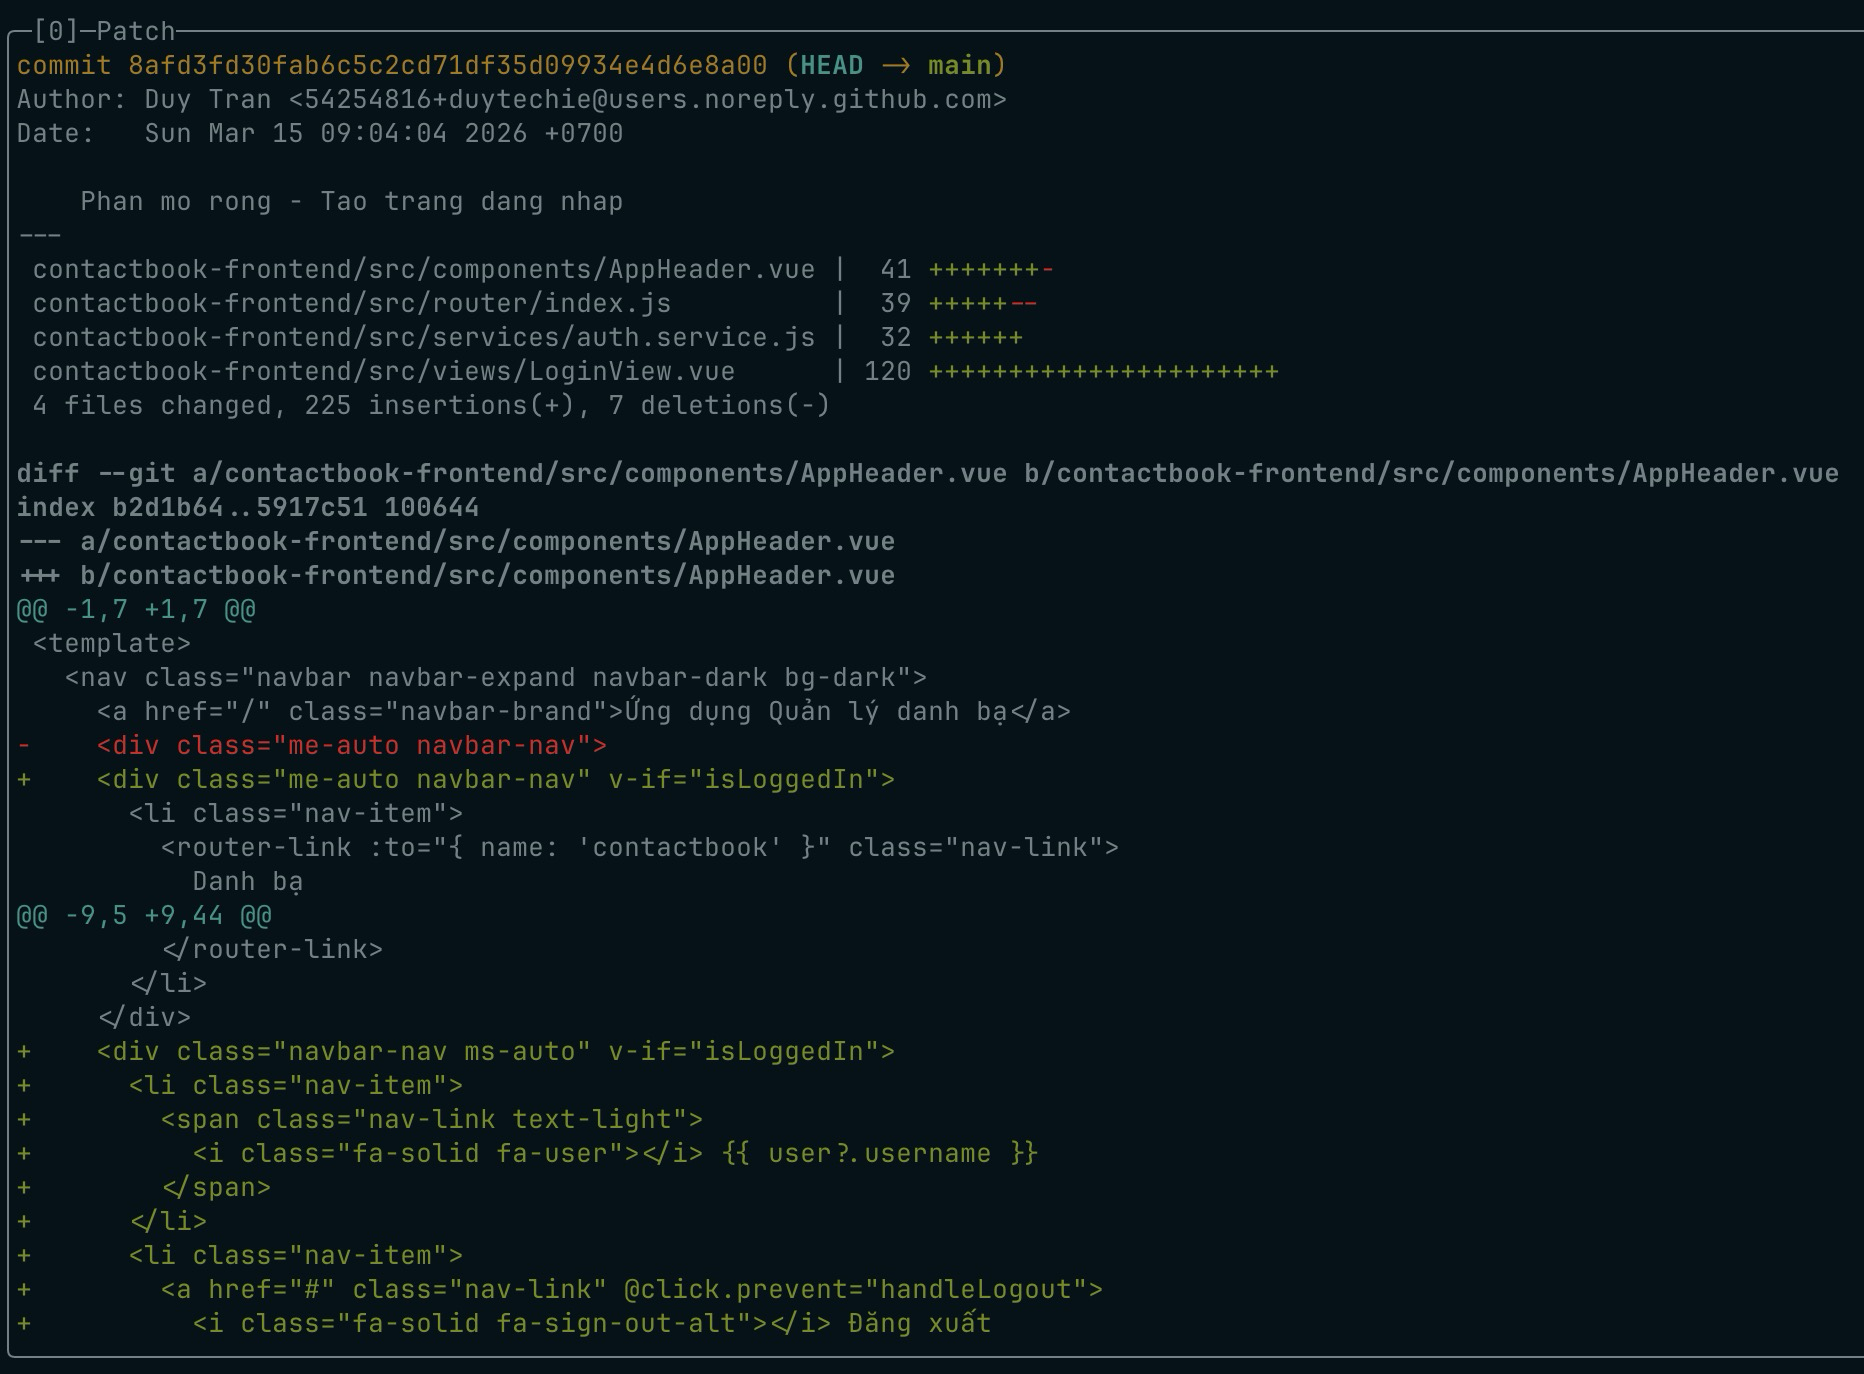
\includegraphics[width=0.8\textwidth]{./assets/login_code.png}
    \caption{Code tạo trang đăng nhập}
    \label{fig:login_code}
\end{figure}

Xem url git commit để biết thêm chi tiết:
\begin{itemize}[noitemsep, topsep=0pt, partopsep=0pt, parsep=0pt]
    \item \href{https://github.com/duytechie/DC24V7X604_TranThanhDuy_FRONTEND/commit/8afd3fd30fab6c5c2cd71df35d09934e4d6e8a00}{8afd3fd}
\end{itemize}

\section{Cấu trúc thư mục dự án đến thời điểm này}

\begin{figure}[H]
    \centering
    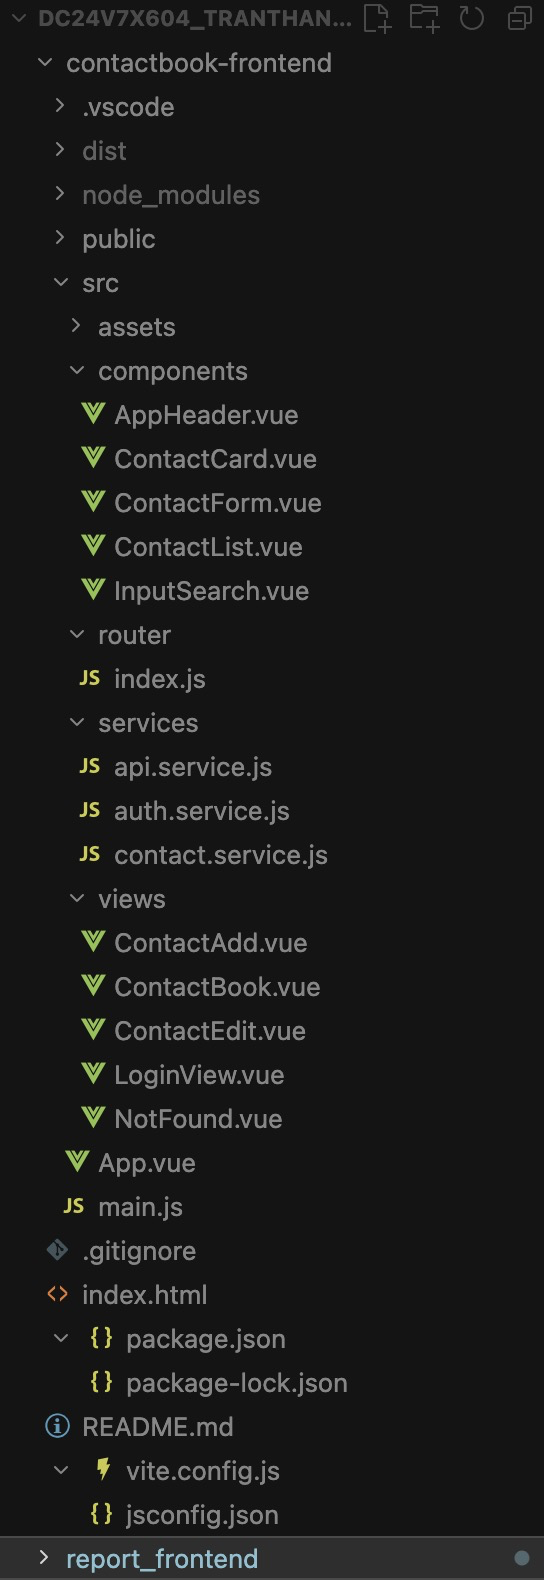
\includegraphics[width=0.4\textwidth]{./assets/project_structure.png}
    \caption{Cấu trúc thư mục dự án}
    \label{fig:project_structure}
\end{figure}

\end{document}